\documentclass{beamer}

\title[Pipelined FFT]{Digital Filter Bank - Pipelined FFT}
\author{Saji Champlin}
\institute{University of Minnesota}
\date{\today}
\subtitle{EE5327 Project Presentation}
\usetheme[secheader]{Boadilla}
\useinnertheme{rectangles}

\usecolortheme{beaver}
\definecolor{darkred}{RGB}{122, 0, 25}

%\setbeamercolor{palette tertiary}{bg=maroon}
\setbeamercolor{titlelike}{bg=gray!15!white}
\setbeamertemplate{itemize items}[default]
\setbeamertemplate{itemize subitem}[circle]
\setbeamertemplate{enumerate items}[default]

\setbeamertemplate{blocks}[rounded]
\setbeamercolor{block body}{bg=gray!15!white}
\setbeamercolor{block title}{bg=gray!15!white}
\setbeamercolor{block body alerted}{bg=gray!15!white}
\setbeamercolor{block title alerted}{bg=gray!15!white}
\setbeamercolor{block body example}{bg=gray!15!white}
\setbeamercolor{block title example}{bg=gray!15!white}

\setbeamercolor{item}{fg=darkred}
\setbeamercolor{subitem}{fg=darkred}
\setbeamercolor{subsubitem}{fg=darkred}

\setbeamertemplate{title page}[default][rounded=true]


% \usefonttheme{professionalfonts}
\beamertemplatenavigationsymbolsempty


\usepackage{amsmath}
% \usepackage[margin=1in]{geometry}
\usepackage[english]{babel}
% \usepackage[shortlabels]{enumitem}
% \usepackage[group-separator={,}]{siunitx}
\usepackage{multicol}
\usepackage{caption}
\usepackage{pdfpages}
\usepackage[outputdir=build]{minted}
\usepackage{tikz}
\usepackage{wrapfig}
\usepackage{pgfplots}
\usepackage{graphicx}
\usepackage{listings}
% \usepackage{biblatex}
% \addbibresource{refs.bib}
\graphicspath{ {./figures/} }
\usetikzlibrary{patterns}

% minted should always be footnotesize and single spaced.
\setminted{fontsize=\footnotesize,baselinestretch=1, frame=lines, breaklines}

% Don't print section numbers
% \setcounter{secnumdepth}{0}
%
% % disable indentation for new paragraphs.
% \setlength{\parindent}{0pt}
% \setlength{\parskip}{0pt plus 0.5ex}


\begin{document}

\frame{\titlepage}

\section{Overview}

\begin{frame}
	\frametitle{Digital Filter Bank and Motivation}
	A digital filter bank is a set of band-pass filters that
	separate a signal into multiple frequency bins.

	The most common way to do this is with an FFT, as
	it converts the signal into frequency domain,
	where performing a band-pass filter is simply selecting
	a range of values on the output.
\end{frame}

\begin{frame}[fragile]
	\frametitle{What is an FFT?}

	An FFT (Fast Fourier Transform) is a very efficient way of computing
	the DFT of a given sequence of values.

	Given $N$ points in a sequence, a naive DFT is $O(N^2)$, whereas an FFT
	is $O(N \log{N})$. This is massive at high values of $N$.
	\pause
	\begin{figure}
		\centering
	\begin{tikzpicture}
		\begin{axis}[ticks=none, axis lines = left, xlabel = \(N\),
				domain=0:100, samples=100, no marks,height=6cm]
			\addplot{x^2};
			\addplot {x * log10(x)};
		\end{axis}
	\end{tikzpicture}
	\end{figure}

\end{frame}


% applications
\begin{frame}
	\frametitle{Applications of FFTs}
	FFTs are very common in DSP applications:

	\begin{itemize}
		\item Radio modulation schemes (OFDM, QAM)
		\item Music "Visualizers", graphic EQs
		\item Radar/Sonar
		\item Noise Spectra/Spectrum Analysis
	\end{itemize}
\end{frame}

\begin{frame}
	\frametitle{How does an FFT work?}
	The classic FFT algorithm is a Cooley-Tukey FFT, which is a divide and conquer algorithm.

	\pause
	This algorithm assumes that $N$ is a power of two. It splits an $N$-point FFT into two $N/2$-point
	FFTs and an additional $O(N)$ multiplications to combine them:

	\pause
	\begin{figure}
		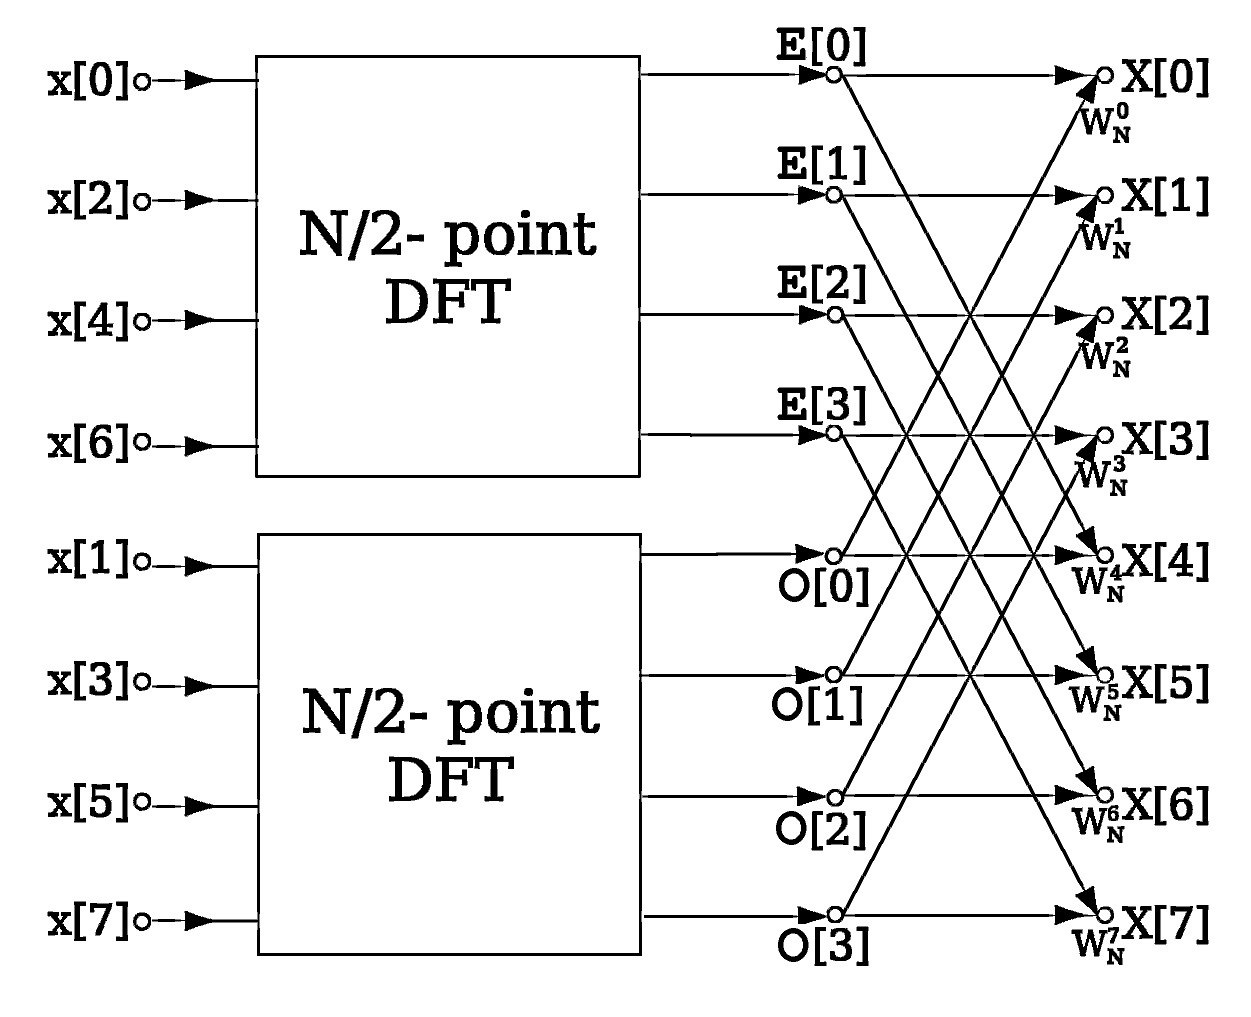
\includegraphics[height=4cm]{DIT-FFT-butterfly.png}
		\caption{By OhArthits - Own work, CC BY 3.0}
		\centering
	\end{figure}

\end{frame}

\begin{frame}
	\frametitle{What is a Pipelined FFT?}
	A pipelined FFT is similar to a pipelined CPU:
	\begin{columns}
		\column{0.38\linewidth}
		\begin{enumerate}
			\item Execution is split into "Stages"
			\pause
			\item Each stage is connected by registers
			\pause
			\item Executing all stages takes 1 cycle and is done in parallel.
		\end{enumerate}
		\column{0.58\linewidth}
		\onslide
		\centering
		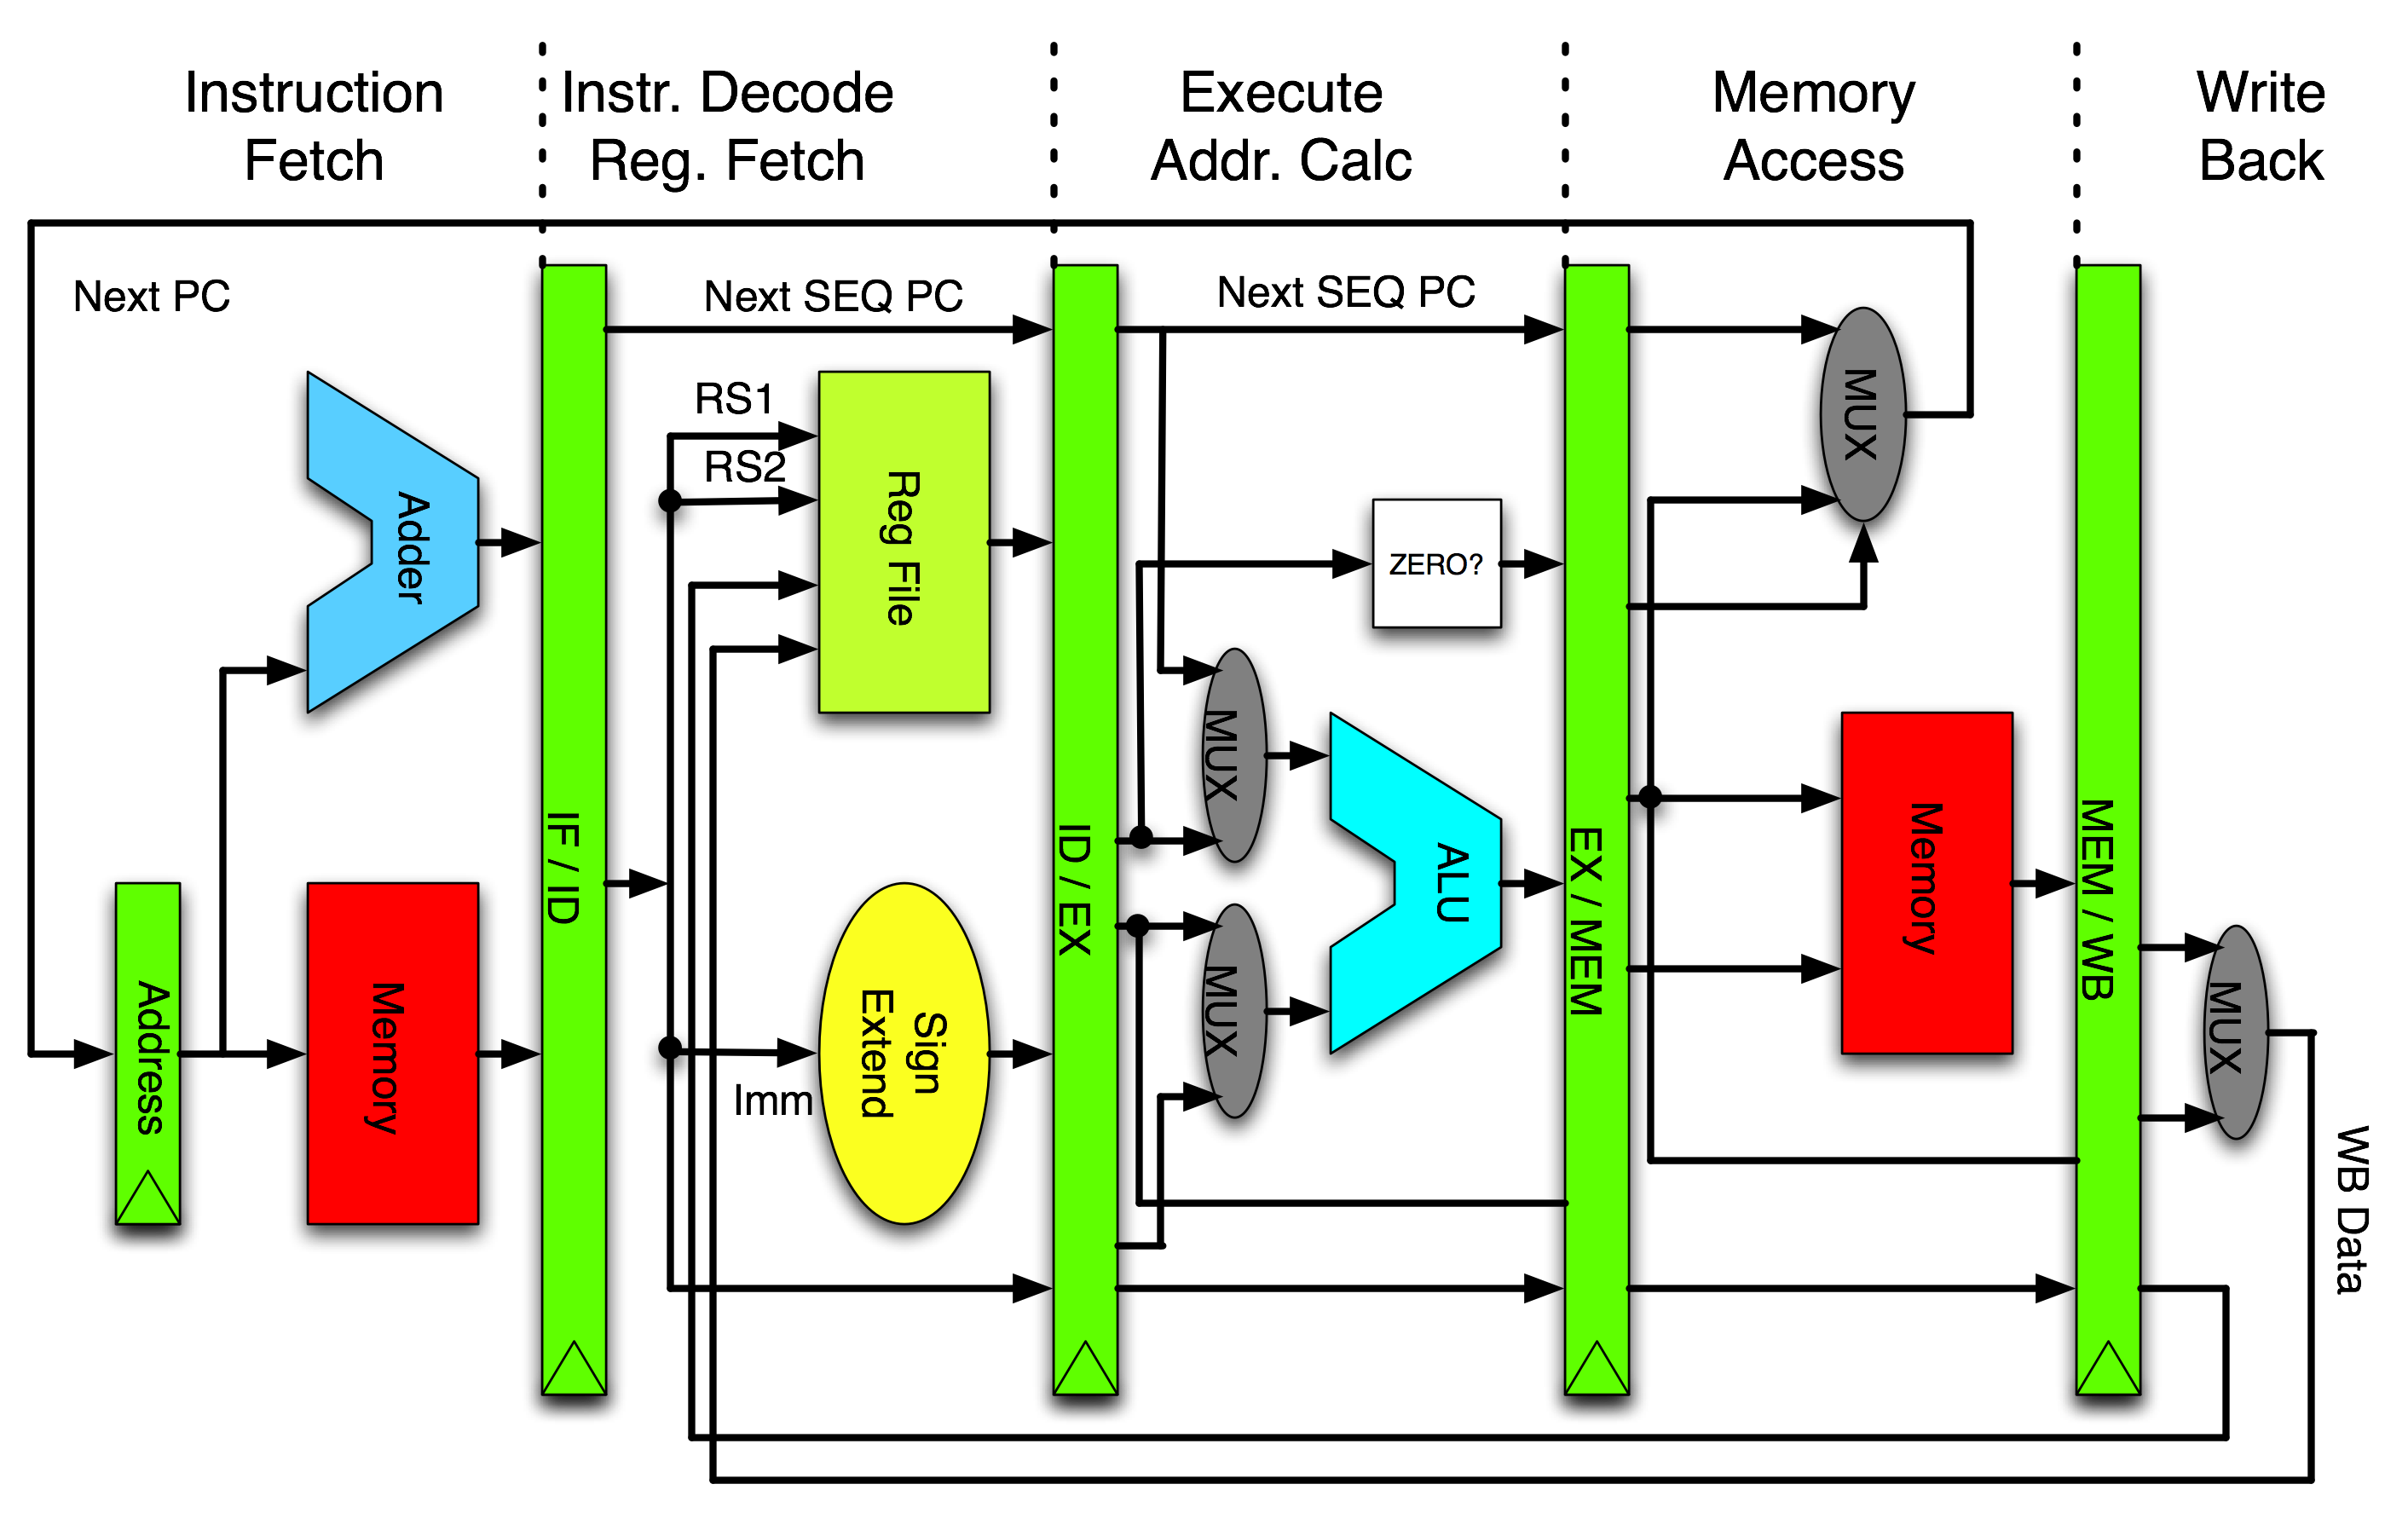
\includegraphics[width=\linewidth]{Pipeline_MIPS.png}
		\captionof{figure}{MIPS 5-stage pipeline example}
	\end{columns}

\end{frame}


\begin{frame}
	\frametitle{How does this work in an FFT?}
	FFTs have $P$ layers where $2^P = N$, so we simply insert registers
	each layer and ensure that a layer can run in a single clock cycle
	\footnote{Single clock isn't a strict requirement, but it does simplify design}.
	\begin{figure}
		\centering
		\begin{tikzpicture}
			\foreach \x in {0,...,3} {
				\draw (0,-\x) node[rectangle,left,draw] (l0_\x) {$x[\x]$};
				\node[circle, draw, minimum size=0.2mm] (l1_\x) at (1,-\x) {}; 
				\node[circle, draw, minimum size=0.2mm] (l2_\x) at (3,-\x) {}; 
				\node[circle, draw, minimum size=0.2mm] (l3_\x) at (5,-\x) {}; 
				\draw [-latex](l0_\x) -- (l1_\x);
				\draw [-latex](l1_\x) -- (l2_\x);
				\draw [-latex](l2_\x) -- (l3_\x);
				\draw [-latex](l3_\x) -- ++(1,0) node[rectangle, right, draw] {$X[\x]$}; 
			}
			
			\draw [-latex](l1_0) -- (l2_1);
			\draw [-latex](l1_1) -- (l2_0);
			\draw [-latex](l1_2) -- (l2_3);
			\draw [-latex](l1_3) -- (l2_2);

			\draw [-latex](l2_0) -- (l3_2);
			\draw [-latex](l2_1) -- (l3_3);
			\draw [-latex](l2_2) -- (l3_0);
			\draw [-latex](l2_3) -- (l3_1);

			\draw [latex-](l2_3) -- ++(0,-1) node[rectangle, below,draw=orange!30] (hi) {registers};
			
			\draw [-latex](hi) -| (l1_3);
			\draw [-latex](hi) -| (l3_3);

			
		\end{tikzpicture}
		\caption{Example DIT FFT structure where $N=4$.}
	\end{figure}
\end{frame}

\section{Design}

\subsection{Architecture}

\begin{frame}
	\frametitle{General structure}
	An FFT is an arrangement of "Butterfly" transforms.
	A butterfly transform is a radix-2 DFT with a complex multiplication factor called
	a "twiddle factor" $w_n^k = e^{-2\pi i k / n}$, where $n$ is the number of points,
	and $k$ is the "position" of the output.
	\begin{align*}
		y_0 &= x_0 + x_1 w_n^k \\
		y_1 &= x_0 - x_1 w_n^k
	\end{align*}
	\pause
	\begin{figure}
		\centering
		\begin{tikzpicture}
			\node [left](x0) at (0,0) {$x_0$};
			\node [left](x1) at (0,-1) {$x_1$};
			\node [right](y0) at (1.5, 0) {$y_0$};
			\node [right](y1) at (1.5, -1) {$y_1$};

			\draw [blue](x0) -- (y0);
			\draw [blue](x0) -- (y1);

			\draw [red](x1) -- (y0);
			\draw [red](x1) -- (y1);

		\end{tikzpicture}
	\end{figure}
	The twiddle factor $w$ is used to rotate the values by a given amount depending on the
	portion of the FFT being calculated.

\end{frame}

\subsection{Complex Multiplier}
\begin{frame}
	\frametitle{Complex Multiplier Math}
	This is a primitive we use in the butterfly module later. It is tricky
	due to being fixed-point and signed. \pause Recall that for complex
	numbers $z = a+bi$ and $y = c + di$, their product is
	\begin{align*}
		z y = (ac + bd) + (ad + bc)i
	\end{align*}
	\pause
	We need fixed point math to store $w$ values. Fixed point multiplication doubles
	the binary point (Q2.14 becomes Q4.28) so we must also account for this in the multiplier.

	\begin{block}{Remark}
		Verilog does not support complex numbers, so I use \texttt{\_re} and
		\texttt{\_im} suffixes to indicate real and imaginary components 
		respectively.
	\end{block}
\end{frame}


\begin{frame}[fragile]
	\frametitle{Complex Multiplier Implementation}
	The crux of the code is as follows 
	(\texttt{WIDTH} and \texttt{FIXED\_POINT} are parameters):
\begin{minted}{verilog}
reg signed [2*WIDTH - 1:0] res_re, res_im;
// the shifted 1 by fixed point -1 is for rounding.
localparam ROUND_FACTOR = 1 << (FIXED_POINT -1);
assign y0_re = res_re[FIXED_POINT + WIDTH-1:FIXED_POINT];
assign y0_im = res_im[FIXED_POINT + WIDTH-1:FIXED_POINT];
always @(posedge clk) begin
  res_re <= a_re * b_re - a_im * b_im + ROUND_FACTOR;
  res_im <= a_re * b_im + a_im * b_re + ROUND_FACTOR;
end
\end{minted}
The round factor is used to improve precision when truncating.
\pause
\begin{block}{Remark}
	All variables/registers are signed. This is to ensure that the Verilog operators
	work correctly (carry-extension mostly).
\end{block}
\end{frame}

\subsection{Butterfly}
\begin{frame}[fragile]
	\frametitle{Butterfly transform}
	Comparatively, the butterfly is simpler, because addition/subtraction does not require
	special behavior for fixed-point math.
\begin{minted}{verilog}
cplx_mul #(.WIDTH(WIDTH)) twiddle_mul (clk, b_re, b_im, twiddle_re, twiddle_im, product_re, product_im);
always @(*) begin
  y0_re = a_re + product_re;
  y0_im = a_im + product_im;
  y1_re = a_re - product_re;
  y1_im = a_im - product_im;
end
\end{minted}
\begin{block}{Note}
I use a combinational always block to prevent needing two clocks to get a result.
\end{block}
\end{frame}

\subsection{Twiddle Factors}

\begin{frame}
	\frametitle{Twiddle Factor Math}
	Twiddle factors can be written in multiple ways:
	\begin{align*}
		w_n^k &= e^{-2\pi i k / n} \\
		      &= \cos(-2\pi k / n) + i\sin(2\pi k / n)
	\end{align*}
	\pause
	\structure{These are periodic functions!}

	We can use this property to compute the factors ahead of time, saving
	time and space for the hardware implementation.
	\begin{block}{Remark}
		Recall that $n$ is the number of points in the FFT, and $k$ is
		the current "position" along those points. There is lots of
		room for optimization of twiddle factors.
	\end{block}
\end{frame}

\begin{frame}[fragile]
	\frametitle{Twiddle Factor Generation}
	We can use a simple python function to generate a single twiddle factor:
\begin{minted}{python}
def twiddle(n,k):
    inner = -2 * math.pi * k / n
    return (math.cos(inner), math.sin(inner))
\end{minted}
This is complemented with a function that converts floats to fixed-point binary strings.
\begin{minted}{python}
def float_to_fixed_binary(num, n_bits, frac_point):
    result = int(num * (2 ** frac_point)) # make the result fixed-point
    if num < 0:
        result = result & ((2 ** n_bits) -1) #2's comp
    return f'{result:0{n_bits}b}' #pad it with zeros to length.
\end{minted}
\end{frame}

\begin{frame}[fragile]
	\frametitle{Loading Twiddle Factors}
	To load the twiddle factors into the module, we use the \texttt{\$readmemb}
	command.
\begin{minted}{verilog}
reg [15:0] tw_f [15:0];
initial $readmemb("rtl/fft8.mem", tw_f);
\end{minted}
\pause
A memory file contains ASCII 0 and 1 without any structure, so we must manually
de-interlace it for complex numbers. Real and imaginary parts are adjacent to
allow for optimization when passing to the butterfly transforms.

\pause
\begin{block}{Remark}
	This is one of the few valid uses of \texttt{initial} in synthesizable
	Verilog.
\end{block}
\end{frame}

\section{Verification}

\subsection{Simulation \& Testbench}
\begin{frame}[fragile]
	\frametitle{Simulation Overview}
	Complex number arithmetic is challenging to do in a Verilog testbench,
	is there a better way to check for correctness?

	\pause
	\structure{Yes!} We can use a tool called \texttt{cocotb} to generate stimulus and
	test module behavior for correct output in Python.

\begin{minted}{python}
@cocotb.test()
async def test_cplx(dut):
    cocotb.start_soon(Clock(dut.clk, 1, 'ns').start())
    await set_terms(dut, 2 + 1j, 3 + 4j)
    await RisingEdge(dut.clk)
    await ReadWrite()
    res = await get_product(dut)
    assert res == (2 + 1j) * (3 + 4j) #2 + 11j
\end{minted}
\captionof{lstlisting}{Simple \texttt{cocotb} test for the complex multiplier}
\end{frame}

\begin{frame}[fragile]
	\frametitle{Cocotb Details}
	\begin{itemize}
\item This test is simple, but supported by helper functions
	that convert python types to inputs for the DUT.
\item \texttt{cocotb} can use multiple simulator backends, including Synopsys VCS,
	as well as open-source software like Verilator or Icarus Verilog.

\item	Because we use floating point in Python, we need to allow for some tolerance
	when comparing with fixed-point values from the DUT:
\begin{minted}{python}
    res = await get_product(dut)
    expected = n1 * n2
    assert math.isclose(res.real,expected.real, abs_tol=0.00390625)
    assert math.isclose(res.imag,expected.imag, abs_tol=0.00390625)
\end{minted}

\item A significant advantage with \texttt{cocotb} is easy randomized tests.


\end{itemize}

\end{frame}

\begin{frame}[fragile]

The output of cocotb for the complex multiplier test suite is as follows:
\begin{minted}{c}
******************************************************************
** TEST                                  STATUS  SIM TIME (ns)  **
******************************************************************
** tests.test_cplx_mul.test_unity         PASS           1.00   **
** tests.test_cplx_mul.test_negation      PASS           1.00   **
** tests.test_cplx_mul.test_imag          PASS           1.00   **
** tests.test_cplx_mul.test_cplx          PASS           1.00   **
** tests.test_cplx_mul.test_rand_ints     PASS         100.00   **
** tests.test_cplx_mul.test_rand_floats   PASS        1000.00   **
******************************************************************
** TESTS=6 PASS=6 FAIL=0 SKIP=0                       1104.01   **
******************************************************************
\end{minted}

\begin{block}{Remark}
	The latter tests use randomly generated complex numbers from Python, chosen
	so that overflow will not occur.
\end{block}
\end{frame}


\begin{frame}
	\frametitle{Sidenote: Should you use \texttt{cocotb}?}
	\structure{You should use \texttt{cocotb} iff:}
	\begin{enumerate}
		\item The inputs and outputs of your modules are 
			non-trivial (fixed-point, complex, etc)
		\item Performing the correct operation in 
			Python is easy (complex multiplication)
		\item A Verilog testbench would use the 
			same operations of your DUT.
	\end{enumerate}
	\structure{You \emph{shouldn't} use \texttt{cocotb} if:}

	\begin{enumerate}
		\item You already have working Verilog testbenches.
		\item Your DUT is not easy to replicate in Python.
	\end{enumerate}
\end{frame}

\begin{frame}
	\frametitle{Waveforms}
	Waveforms are also important to verify approximate timing behavior.
	\begin{figure}
		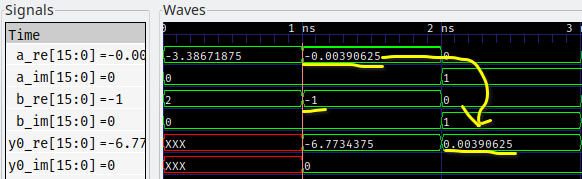
\includegraphics[width=\linewidth]{./../first_report/figures/cplx_mul_waveform.png}
		\caption{Waveforms from the complex multiplier test suite}
		\centering
	\end{figure}
\end{frame}

\begin{frame}[fragile]
	\frametitle{Testing Suite Summary}
	Currently, test cases are written and fully passing for the complex multiplier
	and butterfly modules. The FFT module itself is incomplete and still has several issues.

\end{frame}

\subsection{Synthesis}
\begin{frame}[fragile]
	\frametitle{Basic Synthesis}
A quick synthesis run for the complex multiplier was performed to get preliminary results
for layout parameters and ensure that the Verilog was synthesizable (no unmapped logic).

\begin{minted}{c}
Combinational area:               5936.041318
Buf/Inv area:                      477.282434
Noncombinational area:             292.773895
Macro/Black Box area:                0.000000
Net Interconnect area:            1693.132825

Total cell area:                  6228.815213
Total area:                       7921.948038
\end{minted}
\begin{block}{Remark}
Layout and further optimizations have not been attempted. Furthermore, the FFT itself is still non-functional
however it is simply interconnects and ROM so it should synthesize easily.
\end{block}
\end{frame}

\begin{frame}[fragile]
	\frametitle{Timing estimations}
	On this unoptimized design, I set a timing target of 1ns. It barely failed to reach this.
	Note that 1 nanosecond is insane for most applications.

\begin{minted}{c}
                     Required        Actual
Net                 Transition     Transition     Slack
---------------------------------------------------------
n791                    1.02           1.09       -0.07  (VIOLATED)
    PIN :   U902/A3     1.02           1.09       -0.07  (VIOLATED)
    PIN :   U945/CI     1.02           1.09       -0.07  (VIOLATED)

---------------------------------------------------------
Total                 1                  -0.07
\end{minted}
It may be possible to achieve a 1ns clock with aggressive optimization.
\end{frame}

\section{Summary}

\begin{frame}
	\frametitle{Important takeaways}
	\begin{itemize}
		\item Modular design and testing is important.
		\item Use parameters to allow for flexibility.
		\item Additional tools can provide more robust test suites.
	\end{itemize}

\end{frame}

\begin{frame}
	\frametitle{Remaining Work}
	There are still several things I would like to add in addition to making
	the current version fully functional.
	\begin{itemize}
		\item Fix current 8-point FFT design.
		\item Layout and testability.
		\item Fully-generated FFT (any $N$, width, fixed point).
		\item Variable width/fixed point test suite.
		\item Further optimization of twiddle factors and multipliers.
		\item Mixed-precision (Q4.14 internal registers, Q2.14 I/O)
	\end{itemize}

\end{frame}

\end{document}
